\documentclass[../probability-notes.tex]{subfiles}
\begin{document}
    %%%%%%%%%%%%%%%%%%%%%%%%%%%%%%%%%%%%%%%%%%%%%%%%%%%%%%%%%%%%%%%%%%%%%%%%%%%
    \section{Hypothesis Testing}
    Hypothesis testing is a set of procedures used to test a hypothesis about statistical parameters. Based on the results of the procedure, we decide whether to accept or reject the hypothesis. This can be as simple as deciding whether the mean of a population is more than 1 or not.\newline

    Whenever a hypothesis is accepted, it does not mean that the hypothesis is true, but rather that the data is consistent with it.\newline

    Suppose we have a population that is characterized by the distribution $F_{\theta}$ and we are interested in making statistical comments about the value of the parameters $\theta$. \textbf{The hypothesis that specifies the statement that we are going to test about the parameter is called the null hypothesis} and is denoted by $H_{0}$. Note that the statement of the null hypothesis can either comment on the exact value of the parameter, or comment on an inequality satisfied by the parameter. When the hypothesis completely specifies the distribution, it is called a \emph{simple hypothesis} and in the other case, it is called \emph{composite hypothesis}.\newline

    To test the hypothesis, suppose we have available with us $n$ independent samples from the population. Based on these samples, we must define a $n$ dimensional region $C$ such that if the sample falls in this region, we reject the null hypothesis and vice versa. This region $C$ is called the critical region.
    \begin{align*}
        \text{Reject\:} H_{0} \text{\:if\:} (X_{1}, X_{2}, \ldots, X_{n}) \in C\\
        \text{Acecpt\:} H_{0} \text{\:if\:} (X_{1}, X_{2}, \ldots, X_{n}) \notin C
    \end{align*}

    Two types of errors can result when checking a hypothesis
    \begin{itemize}
        \item \emph{type} $I$ \emph{error}: Reject $H_{0}$ when it is correct
        \item \emph{type} $II$ \emph{error}: Accept $H_{0}$ when it is incorrect
    \end{itemize}

    Since hypothesis testing is about checking if the given data is consistent with the hypothesis, the error we make on rejecting the hypothesis when it is correct should be low. This is consistent with the confidence intervals discussed earlier. We denote \emph{type I error} by $\alpha$ meaning that there is only $\alpha$ chance that the hypothesis will be incorrectly rejected by the test, and is called the level of significance of the test.\newline

    \textbf{A lower significance level or lower $\alpha$ implies that we require stronger evidence against the null hypothesis to reject it.}

    A classical approach while testing the parameters of a population will be to first determine a point estimator of the parameter and then determine the distribution of the said estimator. Hypothesis test will usually involve checking whether the estimator lies in a selcted region, for which we can determine the relevant confidence intervals through the distribution of the estimator.\newline

    
    %%%%%%%%%%%%%%%%%%%%%%%%%%%%%%%%%%%%%%%%%%%%%%%%%%%%%%%%%%%%%%%%%%%%%%%%%%%
    \subsection{Test around Mean of Normal Population}
    %%%%%%%%%%%%%%%%%%%%%%%%%%%%%%%%%%%%%%%%%%%%%%%%%%%%%%%%%%%%%%%%%%%%%%%%%%%
    \subsubsection{Known Variance}\label{sec:mean_normal_known_variance}
    Consider $n$ samples $X_{1}, X_{2}, \ldots, X_{n}$ drawn from a normal distribution with unknown mean $\mu$ and known variance $\sigma^{2}$. We have the following hypothesis
    \begin{align*}
        \text{null hypothesis \:} H_{0}&: \mu = \mu_{0}\\
        \text{alternate hypothesis \:} H_{1}&: \mu \neq \mu_{0}
    \end{align*}

    The sample mean $\overline{X}$ is clearly a natural choice for the estimator of the mean. It is intuitive to define the critical region in such a manner that we reject $H_{0}$ if the estimator is far off from $\mu_{0}$ and vice versa
    \begin{align*}
        C = \{ X_{1}, X_{2}, \ldots X_{n}: |\overline{X} - \mu_{0}| > c\}
    \end{align*}
    for some suitably chosen $c$. We also know that the mean of a normal population has a normal distribution. Hence for some significance level $\alpha$ (\emph{type I error}),
    \begin{align*}
        P_{\mu_{0}}(|\overline{X} - \mu_{0}| > c) = \alpha
    \end{align*}
    where the subscript denotes the fact that the probability is being calculated under the assumption of $\mu = \mu_{0}$. Under this assumption, $\overline{X}$ is normally distributed with mean $mu_{0}$.
    \begin{align*}
        P_{\mu_{0}}(|\frac{\overline{X} - \mu_{0}}{\sigma/\sqrt{n}}| > \frac{c\sqrt{n}}{\sigma}) &= \alpha\\
        2P_{\mu_{0}}(\frac{\overline{X} - \mu_{0}}{\sigma/\sqrt{n}} > \frac{c\sqrt{n}}{\sigma}) &= \alpha
    \end{align*}
    but we know that these are tabulated values
    \begin{align*}
        P(Z > z_{\alpha/2}) &= \alpha/2\\
        \text{or, \:} \frac{c\sqrt{n}}{\sigma} &= z_{\alpha/2}\\
        \text{or, \:} c &= \frac{\sigma z_{\alpha/2}}{\sqrt{n}}
    \end{align*}
    or simply put in terms of the hypothesis test,
    \begin{alignat*}{4}
        \text{Reject\quad} &H_{0} \text{\quad if \quad} &\bigg\lvert \frac{\sqrt{n}}{\sigma}(\overline{X} - \mu_{0}) \big\rvert &> &z_{\alpha/2}\\
        \text{Accept\quad} &H_{0} \text{\quad if\quad} &\big\lvert \frac{\sqrt{n}}{\sigma}(\overline{X} - \mu_{0}) \big\rvert &\leq &z_{\alpha/2}\\
    \end{alignat*}
    where $\alpha$ is the \emph{type I error} and should ideally be low.

    \begin{figure}[h]
    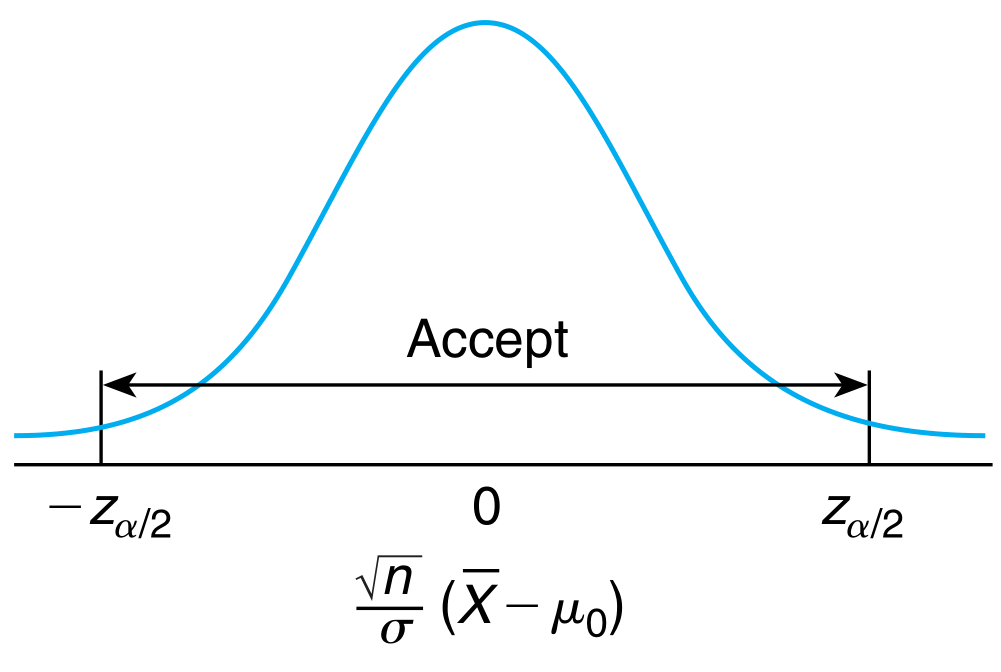
\includegraphics[scale=0.3]{hypo_1}
    \centering
    \caption{Acceptance Region for Hypothesis $\mu=\mu_{0}$}
    \label{fig:hypo_1} %\ref{fig:hypo_1}
    \end{figure}

    %%%%%%%%%%%%%%%%%%%%%%%%%%%%%%%%%%%%%%%%%%%%%%%%%%%%%%%%%%%%%%%%%%%%%%%%%%%
    \subsubsection{p-value}\label{p_value}
    We can also determine an inequality on the significance leve, meaning that $\alpha$ above a certain threshold, we will always reject the null hypothesis and vice versa.\newline
    This threshold is calculated via the probability that the estimator distribution is as large as the test statistic
    \begin{align*}
        P(|Z| > \frac{\sqrt{n}}{\sigma}(\overline{X} - \mu_{0})) = \text{\emph{p-value}}
    \end{align*}
    This \emph{p-value} is interpreted as the threshold for the significance level, i.e., at any significance level less than this value we will accept the null hypothesis and vice versa. This is because the closer the statistic is to zero, the higher the chance that the mean is actually equal to $\mu_{0}$. Thus, a very small \emph{p-value} implies that the statistic is far away from the mean and we can reject $H_{0}$.\newline

    \begin{figure}[h]
    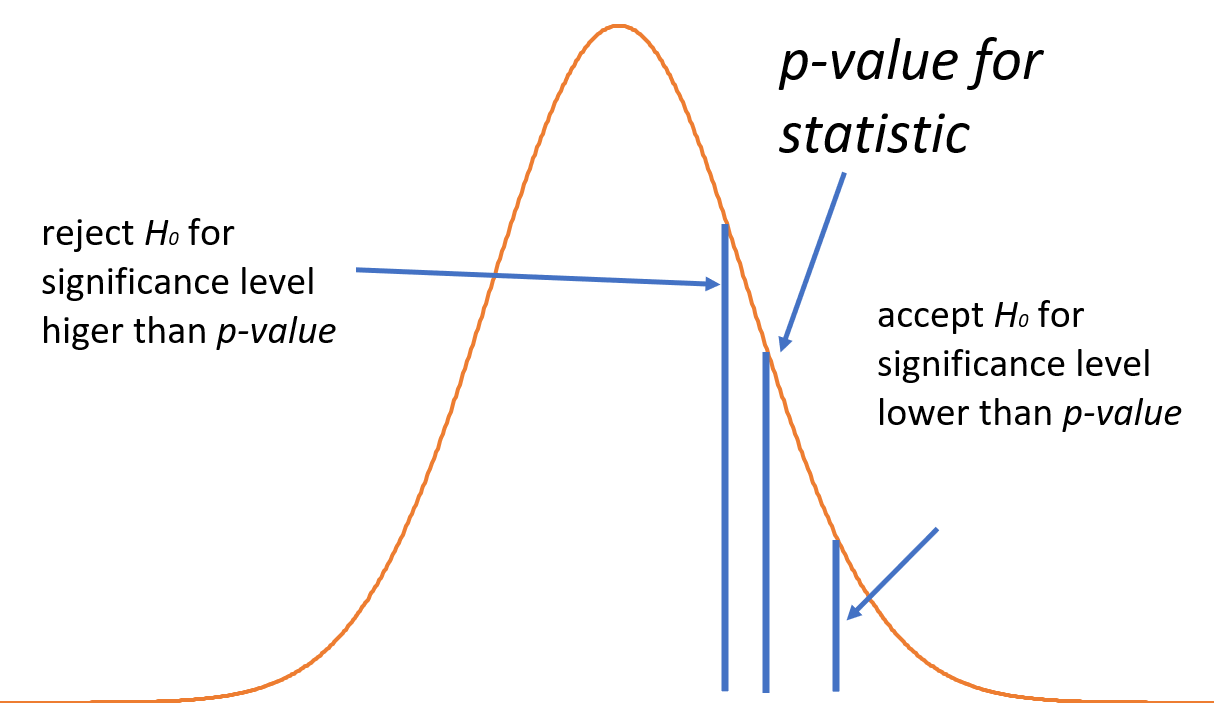
\includegraphics[scale=0.4]{pvalue_1}
    \centering
    \caption{\emph{p-value} and significance levels on a standard normal distribution}
    \label{fig:pvalue_1} %\ref{fig:pvalue_1}
    \end{figure}

    \textbf{Note that \emph{p-value} is not particular to the normal distribution}. We can define it in the context of a t-distribution as well. \emph{p-value} represents the probability value associated with the test statistic under the distribution the test statistic follows.\newline  
    
    Furthermore, if we have a predefined value of the significance level, any \emph{p-value} lower than this level implies it is very likely for the mean to be different, calling for rejecting $H_{0}$. This is visually represented in figure \ref{fig:pvalue_1}.\newline

    We have not yet commented on the \emph{type II error}. Consider $\beta(\mu)$ as probability of accepting $H_{0}$ when the mean is $\mu$
    \begin{align*}
        \beta(\mu) &= P_{\mu}(\text{accepting $H_{0}$ when the mean is $\mu$})\\
        &= P(\text{statistic is \:} \leq z_{\alpha/2})\\
        &= P(|\frac{\sqrt{n}}{\sigma}(\overline{X} - \mu_{0})| \leq z_{\alpha/2})\\
        &= P(-z_{\alpha/2} \leq \frac{\sqrt{n}}{\sigma}(\overline{X} - \mu_{0}) \leq z_{\alpha/2})
    \end{align*}
    But, under the premise that $\mu$ is the correct mean,
    \begin{align*}
        \frac{\overline{X} - \mu}{\sigma/\sqrt{n}} \sim \mathcal{N}(0, 1)
    \end{align*}
    Thus,
    \begin{align*}
        \beta(\mu) &= P(-z_{\alpha/2} - \frac{\sqrt{n}}{\sigma}\mu \leq \frac{\sqrt{n}}{\sigma}(\overline{X} - \mu_{0}) - \frac{\sqrt{n}}{\sigma}\mu \leq z_{\alpha/2} - \frac{\sqrt{n}}{\sigma}\mu)\\
        &= P(-z_{\alpha/2} - \frac{\sqrt{n}}{\sigma}(\mu + \mu_{0}) \leq \frac{\sqrt{n}}{\sigma}(\overline{X} - \mu) \leq z_{\alpha/2} - \frac{\sqrt{n}}{\sigma}(\mu + \mu_{0}))\\
        &= \Phi(z_{\alpha/2} - \frac{\sqrt{n}}{\sigma}(\mu - \mu_{0})) - \Phi(-z_{\alpha/2} - \frac{\sqrt{n}}{\sigma}(\mu - \mu_{0}))\\
        &= \Phi(\frac{\sqrt{n}}{\sigma}(\mu_{0} - \mu) +z_{\alpha/2}) - \Phi(\frac{\sqrt{n}}{\sigma}(\mu_{0} - \mu) -z_{\alpha/2})\\
    \end{align*}
    where $\Phi$ is the standard normal cumulative distribution function.\newline
    $\beta(\mu)$ is called the Operating Charectistic. The value of this function is only dependent on the gap between $\mu_{0}$ and $\mu$. For a fix $\alpha$, as the gap grows, we move away from the centre of the standard normal. As such, the difference in the two terms of $\beta(\mu)$ keeps decreasing. It is maximum when $\mu = \mu_{0}$.

    \begin{figure}[h]
    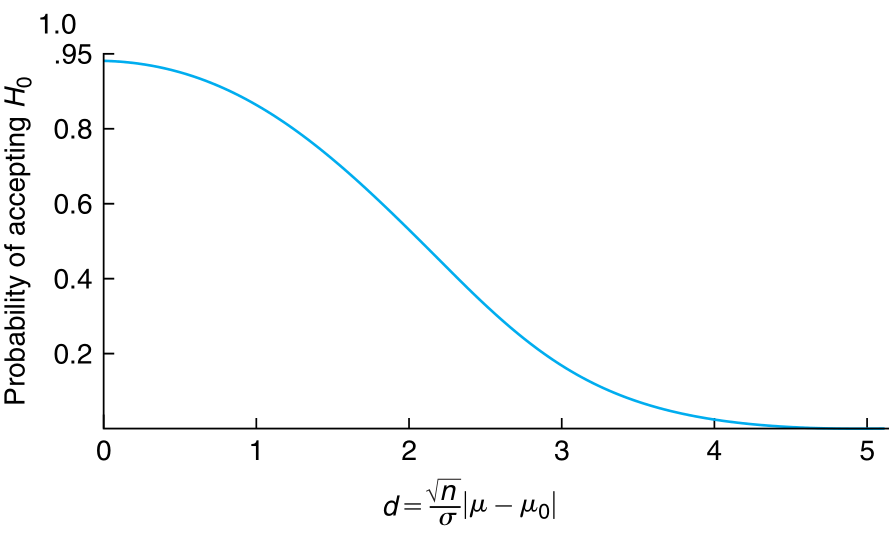
\includegraphics[scale=0.3]{hypo_2}
    \centering
    \caption{Curve of $\beta(\mu)$ for a fixed $\alpha$}
    \label{fig:hypo_2} %\ref{fig:hypo_2}
    \end{figure}

    The function $1 - \beta(\mu)$ is called the \emph{power function} and is the probability of rejection of $H_{0}$ when the true mean is $\mu$. This function is useful in calculating the value of the sample size so that the probability of accepting $H_{0}: \mu = \mu_{0}$ when the true mean is $\mu_{1}$ is $\beta$. We solve the equation $\beta(\mu_{1}) = \beta$ and try to guess the value of $n$ because analytical solution is not possible.

    \begin{align*}
         n \approx \frac{(z_{\alpha/2} + z_{\beta})^{2} \sigma^{2}}{(\mu_{1} - \mu_{0})^{2}}
    \end{align*}
    is the approximate solution assuming $\alpha$ is negligible.


    %%%%%%%%%%%%%%%%%%%%%%%%%%%%%%%%%%%%%%%%%%%%%%%%%%%%%%%%%%%%%%%%%%%%%%%%%%%
    \subsubsection{One Sided Test}
    In one sided test, we test the equality of the mean with a fixed value vs a single sided inequality of the mean being larger than, or smaller than that fixed value.
    \begin{align*}
        \text{null hypothesis \:} H_{0}&: \mu = \mu_{0}\\
        \text{alternate hypothesis \:} H_{1}&: \mu > \mu_{0}
    \end{align*}

    Note that the variance of the distribution is known in this case. Clearly, the critical region (rejection region) is one where the large values of $\mu$ are unlikely
    \begin{align*}
        C = {X_{1}, \ldots, X_{n}: \overline{X} - \mu_{0} > c}
    \end{align*}
    for some constant $c$ chosen based on the significance level $\alpha$. Equivalently,
    \begin{align*}
        P(\frac{\overline{X} - \mu_{0}}{\sigma/\sqrt{n}} > z_{\alpha}) &= \alpha\\
        \text{or, \:} \overline{X} &> z_{\alpha}\frac{\sigma}{\sqrt{n}} + \mu_{0}
    \end{align*}

    is the rejection region based on the sample mean.

    \begin{alignat*}{4}
        \text{Reject\quad} &H_{0} \text{\quad if \quad} &\frac{\sqrt{n}}{\sigma}(\overline{X} - \mu_{0}) &> &z_{\alpha}\\
        \text{Accept\quad} &H_{0} \text{\quad if\quad} &\frac{\sqrt{n}}{\sigma}(\overline{X} - \mu_{0}) &\leq &z_{\alpha}\\
    \end{alignat*}

    The \emph{p-value} is similarly calculated as the probability that the standard normal is at least as large as this test statistic. Similar to the two sided test, operating characteristic curve can be defined
    \begin{align*}
        \beta(\mu) &= P(\text{Accepting\:} H_{0})\\
        &= P(\overline{X} \leq z_{\alpha}\frac{\sigma}{\sqrt{n}} + \mu_{0})\\
        &= P(\frac{\overline{X} - \mu}{\sigma/\sqrt{n}} \leq z_{\alpha} + \frac{\mu_{0} - \mu}{\sigma/\sqrt{n}})\\
        &= P(Z \leq z_{\alpha} + \frac{\mu_{0} - \mu}{\sigma/\sqrt{n}})
    \end{align*}
    where $Z$ is the standard normal.\newline

    \paragraph{Special Note} The tests discussed above have been derived under the assumption that the sample mean has a normal distribution. But, by central limit theorem, the sample mean of any large population will tend towards a normal distribution. Hence, the hypothesis tests will remain valid provided the population has known variance $\sigma$.

    %%%%%%%%%%%%%%%%%%%%%%%%%%%%%%%%%%%%%%%%%%%%%%%%%%%%%%%%%%%%%%%%%%%%%%%%%%%
    \subsubsection{Unknown Variance}\label{mean_normal_unknown_variance}
    We proceed in a manner similar to the known variance case but use sample variance instead. Recall
    \begin{align*}
        \sqrt{n} \frac{\overline{X} - \mu_{0}}{S} \sim T_{n-1}
    \end{align*}
    which is a t-distributed random variable with $n-1$ degrees of freedom. Since t-distribution also has specially defined values $t_{\alpha, n-1}$ similar to $z_{\alpha}$, we can simply use the following 2-sided tests at significance level $\alpha$
    \begin{alignat*}{4}
        \text{Reject\quad} &H_{0} \text{\quad if \quad} &\bigg \lvert\frac{\sqrt{n}}{S}(\overline{X} - \mu_{0}) \bigg\rvert &> &t_{\alpha/2, n-1}\\
        \text{Accept\quad} &H_{0} \text{\quad if\quad} &\bigg \lvert\frac{\sqrt{n}}{S}(\overline{X} - \mu_{0}) \bigg\rvert &\leq &t_{\alpha/2, n-1}\\
    \end{alignat*}

    Further, \emph{p-values} are defined using the same statistic $\sqrt{n}(\overline{X} - \mu_{0})/S$ and for any significance level which is less than the \emph{p-value} probability that the t-statistic is greater than this statistic $\sqrt{n}(\overline{X} - \mu_{0})/S$, we will reject $H_{0}: \mu = \mu_{0}$. We accept the null hypothesis when the significance level is larger than the \emph{p-value}.\newline

    Similar to the known variance case, we have the one sided tests defined as below
    \begin{align*}
        H_{0}: \mu \leq \mu_{0} \quad \text{versus} \quad H_{1}: \mu > \mu_{0}
    \end{align*}
    \begin{alignat*}{4}
        \text{Reject\quad} &H_{0} \text{\quad if \quad} &\frac{\sqrt{n}}{S}(\overline{X} - \mu_{0}) &> &t_{\alpha, n-1}\\
        \text{Accept\quad} &H_{0} \text{\quad if\quad} &\frac{\sqrt{n}}{S}(\overline{X} - \mu_{0}) &\leq &t_{\alpha, n-1}\\
    \end{alignat*}
    and the other side
    \begin{align*}
        H_{0}: \mu \geq \mu_{0} \quad \text{versus} \quad H_{1}: \mu < \mu_{0}
    \end{align*}
    \begin{alignat*}{4}
        \text{Reject\quad} &H_{0} \text{\quad if \quad} &\frac{\sqrt{n}}{S}(\overline{X} - \mu_{0}) &< &-t_{\alpha, n-1}\\
        \text{Accept\quad} &H_{0} \text{\quad if\quad} &\frac{\sqrt{n}}{S}(\overline{X} - \mu_{0}) &\geq &-t_{\alpha, n-1}\\
    \end{alignat*}
    and we can calculate the \emph{p-value} as well in the above cases using the test statistic.\newline

    
    %%%%%%%%%%%%%%%%%%%%%%%%%%%%%%%%%%%%%%%%%%%%%%%%%%%%%%%%%%%%%%%%%%%%%%%%%%%
    \subsection{Testing Equality of Means of Two Normal Populations}
    %%%%%%%%%%%%%%%%%%%%%%%%%%%%%%%%%%%%%%%%%%%%%%%%%%%%%%%%%%%%%%%%%%%%%%%%%%%
    \subsubsection{Known Variances} \label{mean_diff_normal_known_variance}
    Consider the two populations as
    \begin{align*}
        X_{1}, X_{2}, \ldots, X_{n} &\sim \mathcal{N}(\mu_{x}, \sigma_{x}^{2})\\
        Y_{1}, Y_{2}, \ldots, Y_{m} &\sim \mathcal{N}(\mu_{y}, \sigma_{y}^{2})
    \end{align*}

    Then, the difference in the sample means will itself be a normal distribution (since it is the difference of two normals), and the test statistic can be defined as below
    \begin{align*}
        \overline{X} - \overline{Y} \sim \mathcal{N}(\mu_{x} - \mu_{y}, \sqrt{\frac{\sigma_{x}^{2}}{n} + \frac{\sigma_{y}^{2}}{m}})\\
        T = \frac{(\overline{X} - \overline{Y}) - (\mu_{x} - \mu_{y})}{\sqrt{\frac{\sigma_{x}^{2}}{n} + \frac{\sigma_{y}^{2}}{m}}} \sim \mathcal{N}(0, 1)
    \end{align*}

    when $H_{0}$ is true,
    \begin{align*}
        T = \frac{(\overline{X} - \overline{Y})}{\sqrt{\frac{\sigma_{x}^{2}}{n} + \frac{\sigma_{y}^{2}}{m}}} \sim \mathcal{N}(0, 1)
    \end{align*}
    and we compare the following hypotheses
    \begin{alignat*}{3}
        &H_{0}: \mu_{x} = \mu_{y} \quad &\text{versus} \quad &H_{1}: \mu_{x} \neq \mu_{y}\\
        \text{or,} \quad &H_{0}: \mu_{x} - \mu_{y} = 0 \quad &\text{versus} \quad &H_{1}: \mu_{x} - \mu_{y} \neq 0
    \end{alignat*}
    we reject $H_{0}$ when the difference between the means is large, i.e., $H_{0}$ is testing whether the test statistic is close to zero or not

    \begin{alignat*}{4}
        \text{Reject\quad} &H_{0} \text{\quad if \quad} &T &> &z_{\alpha/2}\\
        \text{Accept\quad} &H_{0} \text{\quad if\quad} &T &\leq &z_{\alpha/2}
    \end{alignat*}
    where the variances of both the populations are known.\newline

    In a very similar fashion, the hypthesis testing rules for one sided test can be derived.\newline
    For
    \begin{align*}
        H_{0}: \mu_{x} \leq \mu_{y} \quad \text{versus} \quad H_{1}: \mu_{x} > \mu_{y}
    \end{align*}
    We reject $H_{0}$ when the difference $\mu_{x} - \mu_{y}$ is highly positive
    \begin{alignat*}{4}
        \text{Reject\quad} &H_{0} \text{\quad if \quad} &\frac{(\overline{X} - \overline{Y})}{\sqrt{\frac{\sigma_{x}^{2}}{n} + \frac{\sigma_{y}^{2}}{m}}} &> &z_{\alpha}\\
        \text{Accept\quad} &H_{0} \text{\quad if\quad} &\frac{(\overline{X} - \overline{Y})}{\sqrt{\frac{\sigma_{x}^{2}}{n} + \frac{\sigma_{y}^{2}}{m}}} &\leq &z_{\alpha}
    \end{alignat*}

    For the other side of the test, we use the same criteria as above, but switching the sets $X$ and $Y$.

    
    %%%%%%%%%%%%%%%%%%%%%%%%%%%%%%%%%%%%%%%%%%%%%%%%%%%%%%%%%%%%%%%%%%%%%%%%%%%
    \subsubsection{Unknown but Equal Variances}
    We consider the same two populations of $Xs$ and $Ys$, but this time the variances are unknown. for simplicity of analysis, we assume that the unknown variances are same
    \begin{align*}
        \sigma_{x} = \sigma_{y} = \sigma
    \end{align*}

    From section \ref{mean_diff_normal}, we know
    \begin{align*}
        S_{p}^{2} = \frac{(n-1)S_{1}^{2} + (m-1)S_{2}^{2}}{n + m - 2}\\
        \frac{(\overline{X} - \overline{Y}) - (\mu_{x} - \mu_{y})}{\sqrt{\frac{\sigma_{x}^{2}}{n} + \frac{\sigma_{y}^{2}}{m}}} \div \frac{S_{p}}{\sigma} \sim t_{n+m-2}
    \end{align*}

    If $H_{0}$ is true, $\mu_{x} = \mu_{y}$ and we have
    \begin{align*}
        T = \frac{(\overline{X} - \overline{Y})}{S_{p}\sqrt{\frac{1}{m} + \frac{1}{n}}} \sim t_{n+m-2}
    \end{align*}

    and we have the critical region defined as
    \begin{alignat*}{4}
        \text{Reject\quad} &H_{0} \text{\quad if \quad} &T &> &t_{\alpha/2, n+m-2}\\
        \text{Accept\quad} &H_{0} \text{\quad if\quad} &T &\leq &t_{\alpha/2, n+m-2}
    \end{alignat*}

    and for the one sided hypothesis
    \begin{align*}
        H_{0}: \mu_{x} \leq \mu_{y} \quad \text{versus} \quad H_{1}: \mu_{x} > \mu_{y}
    \end{align*}
    We reject $H_{0}$ when the difference $\mu_{x} - \mu_{y}$ is highly positive
    \begin{alignat*}{4}
        \text{Reject\quad} &H_{0} \text{\quad if \quad} &T &> &t_{\alpha, n+m-2}\\
        \text{Accept\quad} &H_{0} \text{\quad if\quad} &T &\leq &z_{\alpha, n+m-2}
    \end{alignat*}    


    %%%%%%%%%%%%%%%%%%%%%%%%%%%%%%%%%%%%%%%%%%%%%%%%%%%%%%%%%%%%%%%%%%%%%%%%%%%
    \subsubsection{Unknown and Unequal Variances}
    We consider the natural test statistic as follows
    \begin{align*}
        \frac{(\overline{X} - \overline{Y}) - (\mu_{x} - \mu_{y})}{\sqrt{\frac{S_{x}^{2}}{n} + \frac{S_{y}^{2}}{m}}}
    \end{align*}
    Even when $H_{0}$ is true, the above is not a simple distribution to solve for. If we make the additional assumption that $n$ and $m$ are large, then
    \begin{align*}
        \frac{(\overline{X} - \overline{Y})}{\sqrt{\frac{S_{x}^{2}}{n} + \frac{S_{y}^{2}}{m}}} \sim \mathcal{N}(0, 1)
    \end{align*}
    and the same criteria for accepting and rejecting $H_{0}$ discussed in section \ref{mean_diff_normal_known_variance} are applicable, but after replacing population variances with sample variances.\newline


    %%%%%%%%%%%%%%%%%%%%%%%%%%%%%%%%%%%%%%%%%%%%%%%%%%%%%%%%%%%%%%%%%%%%%%%%%%%
    \subsubsection{Unknown and Unequal Variances}
    Suppose we want to observe the change in a quantity in a sample, after some kind of intervention. A simple example can be change in the mileage of a car after installation of a catalytic converter. Suppose we have $n$ samples with us, and for each of the sample, we associate $X_{i}$ with the measurement of the quantity before intervention and $Y_{i}$ with the quantity post intervention. Note that $X_{i}$ is not independent of $Y_{i}$ because they come from the same $i^{th}$ sample. Hence, the test discussed in section \ref{mean_diff_normal_known_variance} is not applicable.\newline

    Instead, we consider the quantity $W = X - Y$ and assume that $W_{i}$ come from a normal population. We can then consider the hypothesis
    \begin{align*}
        H_{0}: \mu_{w} = 0 \quad \text{versus} \quad H_{1}: \mu_{w} \neq 0
    \end{align*}

    Using the results derived in section \ref{mean_normal_unknown_variance}, we have
    \begin{alignat*}{4}
        \text{Reject\quad} &H_{0} \text{\quad if \quad} &\sqrt{n}\frac{\overline{W}}{S_{w}} &> &t_{\alpha/2, n-1}\\
        \text{Accept\quad} &H_{0} \text{\quad if\quad} &\sqrt{n}\frac{\overline{W}}{S_{w}} &\leq &t_{\alpha/2, n-1}
    \end{alignat*}

    One sided tests can be derived in exactly the same manner as section \ref{mean_normal_unknown_variance} and the concepts discussed in \ref{p_value} still hold true.


    %%%%%%%%%%%%%%%%%%%%%%%%%%%%%%%%%%%%%%%%%%%%%%%%%%%%%%%%%%%%%%%%%%%%%%%%%%%
    \subsection{Tests around Variance of Normal Population}
    For a $n$ sized sample of independent observations from a normal population, we are interested in checking
    \begin{align*}
        H_{0}: \sigma^{2} = \sigma_{0}^{2} \quad \text{versus} \quad \sigma^{2} \neq \sigma_{0}^{2}
    \end{align*}

    Recall from section \ref{dist_for_normal}
    \begin{align*}
        \frac{(n-1)S^{2}}{\sigma^{2}} \sim \chi_{n-1}^{2}
    \end{align*}

    Then if $H_{0}$ is true, our test statistic
    \begin{align*}
        TS = \frac{(n-1)S^{2}}{\sigma_{0}^{2}} \sim \chi_{n-1}^{2}
    \end{align*}

    and from the test simply becomes
    \begin{alignat*}{2}
        \text{Accept\quad} &H_{0} \quad &\text{if} \quad \chi_{1-\alpha/2, n-1}^{2} \leq TS \leq \chi_{\alpha/2, n-1}^{2}\\
        \text{Reject\quad} &H_{0} \quad &\text{otherwise}
    \end{alignat*}

    One sided test can be done in a similar manner, comparing with $\chi_{1-\alpha, n-1}^{2}$ or $\chi_{\alpha, n-1}^{2}$ based on which side we want to reject $H_{0}$.\newline

    %%%%%%%%%%%%%%%%%%%%%%%%%%%%%%%%%%%%%%%%%%%%%%%%%%%%%%%%%%%%%%%%%%%%%%%%%%%
    \subsubsection{Comparing Variance of Two Normal Populations}
    We are interested in comparing
    \begin{align*}
        H_{0}: \sigma_{x}^{2} = \sigma_{y}^{2} \quad \text{versus} \quad \sigma_{x}^{2} \neq \sigma_{y}^{2}
    \end{align*}

    Recall that the ratio of sample variance with population variance is t-distributed, and the ratio of two t-distributed variables has an F-distribution. Hence, when $H_{0}$ is true,
    \begin{align*}
        TS = \frac{S_{x}^{2}}{S_{y}^{2}} \sim F_{n-1, m-1}
    \end{align*}

    Noting that F-distribution is always positive, the region for accepting $H_{0}$ simply become
    \begin{alignat*}{2}
        \text{Accept\quad} &H_{0} &\text{\quad if} \quad F_{1-\alpha/2, n-1, m-1} \leq TS \leq F_{\alpha/2, n-1, m-1}\\
        \text{Reject\quad} &H_{0} &\text{\quad otherwise}
    \end{alignat*}

    %%%%%%%%%%%%%%%%%%%%%%%%%%%%%%%%%%%%%%%%%%%%%%%%%%%%%%%%%%%%%%%%%%%%%%%%%%%
    \subsection{Tests around Bernoulli Population}
    Suppose we have a set of $n$ samples and we want to test how many of them satisfy a property (or equivalently, success). Let $p$ be the fraction of population satisfying he property and we want to check if this equals $p_{0}$
    \begin{align*}
        H_{0}: p \leq p_{0} \quad \text{versus} \quad p > p_{0}
    \end{align*}

    i.e., we reject this batch if the size of sample not satisfying the property (defective) is more than some predefined quantity/significance $p_{0}$.\newline

    We reject when the defectives in the sample ($X$) are more than a threshold $k$
    \begin{align*}
        P(X \geq k) = \sum_{i=k}^{n} \binom{n}{i} = \sum_{i=k}^{n} p^{i}(1-p)^{n-i}
    \end{align*}

    which is an increasing function in $p$. Hence, when $H_{0}$ is true,
    \begin{align*}
        P(X \geq k) \leq \sum_{i=k}^{n} p_{0}^{i}(1-p_{0})^{n-i}
    \end{align*}

    and we reject when $X \geq k^{*}$ depending on the significance level $\alpha$
    \begin{align*}
        k^{*} = \text{minimum}\quad k \quad \text{where} \quad \sum_{i=k}^{n} p_{0}^{i}(1-p_{0})^{n-i} \leq \alpha
    \end{align*}
    because there can be multiple $k$ which satisfy the above equation, and we want to reject $H_{0}$ as soon as the number of defectives in sample $X$ is more than the minimum $k$.\newline

    The test can also be done using \emph{p-value}
    \begin{align*}
        \text{\emph{p-value}} &= P(Bin(n, p_{0}) \geq x)\\
        &= \sum_{i=x}^{n}p_{0}^{i}(1-p_{0})^{n-i}
    \end{align*}

    where $x$ is the count of defects in the sample. We reject $H_{0}$ at any $\alpha >$ \emph{p-value} since in that situation the number of defects required will be much less than $x$.

    For large $n$, $X$ will behave like a normal distribution and when $H_{0}$ is true,
    \begin{align*}
        \frac{X - np_{0}}{\sqrt{np_{0}(1-p_{0})}} \sim \mathcal{N}(0,1)
    \end{align*}

    and criteria discussed in section \ref{sec:mean_normal_known_variance} hold.\newline




\end{document}